\documentclass[UTF8]{ctexart}   %中文article文档类型排版,UTF8编码
\usepackage{amsmath}            %调用公式宏包
\usepackage{graphicx}           %插入图片宏包
\usepackage{hyperref}
\usepackage{fontspec}
\hypersetup{
			colorlinks,
			linkcolor=red,
			anchorcolor=blue,
			citecolor=green,
			CJKbookmarks=True
			}




\newtheorem{thm}{定理}               %定义标题为定理的定理类环境thm
\newcommand\degree{^\circ}           %定义新命令degree用来写角度的



\begin{document}



\title{这是标题}
\date{\today}
\author{史学睿}
\maketitle

这里是正文



\begin{equation}
	a_v=b
\end{equation}

\begin{figure}[!ht]\centering %添加图片环境的配置
	   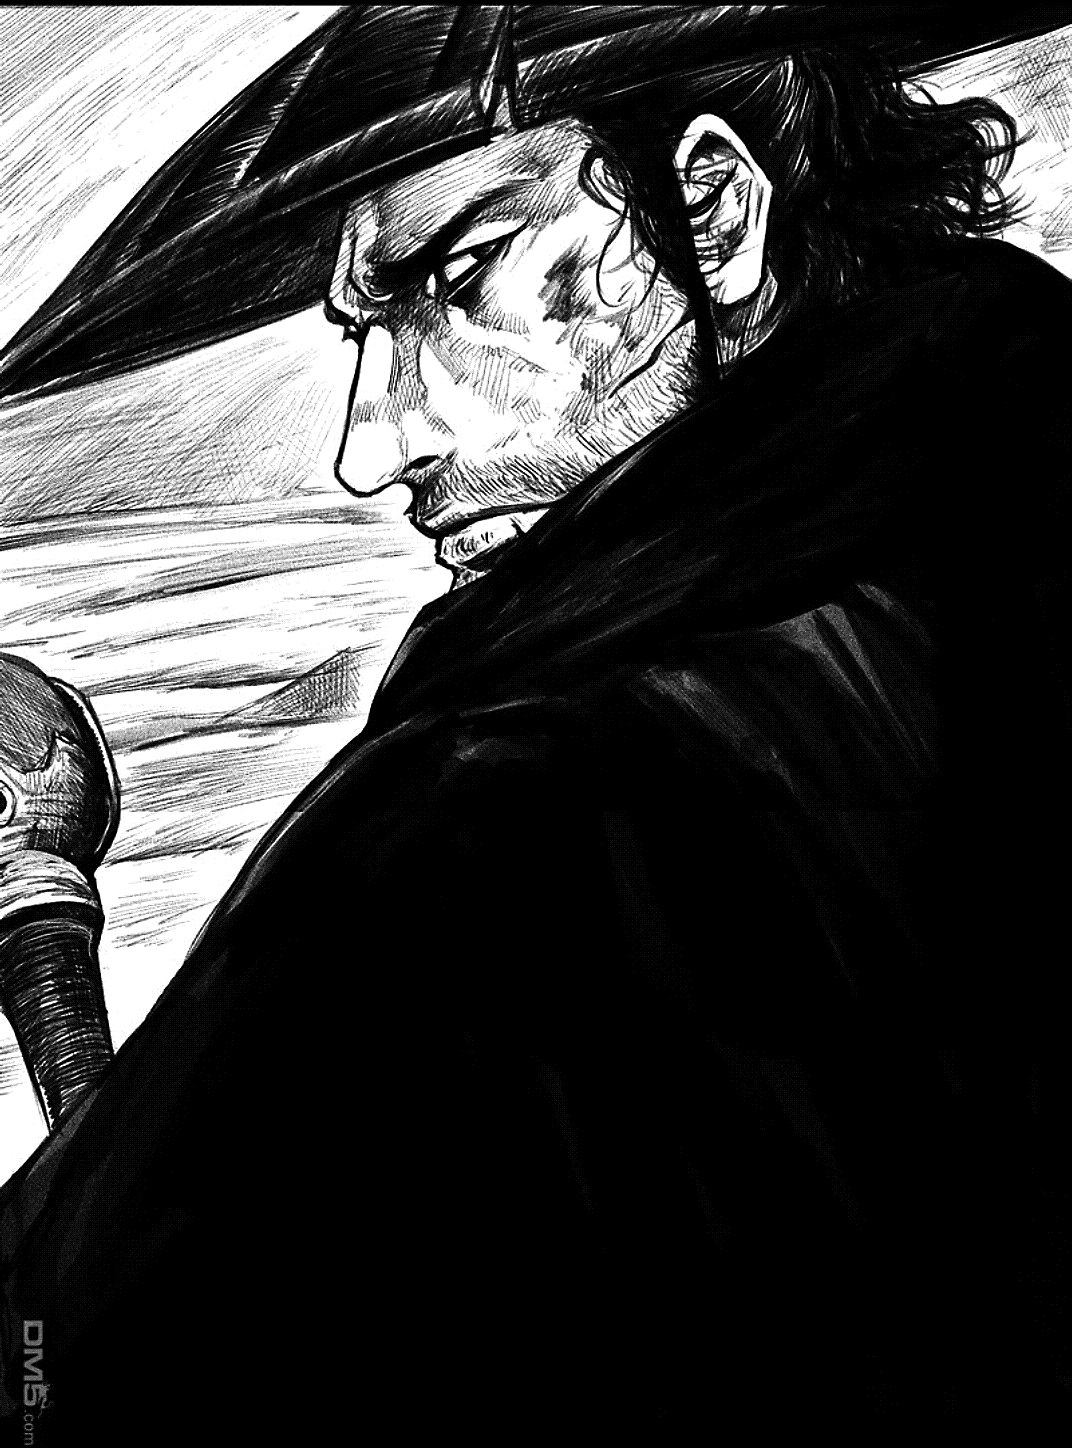
\includegraphics[width=0.30\textwidth]{Image/xiantu.jpg}       %添加图片
	   \caption{}    %图片下面的文字说明
\end{figure}

\end{document}
